\documentclass{article}

\usepackage{amsmath, amsthm, amssymb, amsfonts}
\usepackage{thmtools}
\usepackage{graphicx}
\usepackage{setspace}
\usepackage{geometry}
\usepackage{float}
\usepackage{hyperref}
\usepackage[utf8]{inputenc}
\usepackage[english]{babel}
\usepackage{framed}
\usepackage[dvipsnames]{xcolor}
\usepackage{tcolorbox}
\usepackage{physics}
\DeclareMathOperator{\grd}{grad}
\DeclareMathOperator{\area}{Area}
\colorlet{LightGray}{White!90!Periwinkle}
\colorlet{LightOrange}{Orange!15}
\colorlet{LightGreen}{Green!15}

\newcommand{\HRule}[1]{\rule{\linewidth}{#1}}

\declaretheoremstyle[name=Theorem,]{thmsty}
\declaretheorem[style=thmsty,numberwithin=section]{theorem}
%\tcolorboxenvironment{theorem}{colback=LightGray}

\declaretheoremstyle[name=Proposition,]{prosty}
\declaretheorem[style=prosty,numberlike=theorem]{proposition}
\tcolorboxenvironment{proposition}{colback=LightOrange}

\declaretheoremstyle[name=Principle,]{prcpsty}
\declaretheorem[style=prcpsty,numberlike=theorem]{principle}
\tcolorboxenvironment{principle}{colback=LightGreen}

\setstretch{1.2}
\geometry{
    textheight=9in,
    textwidth=5.5in,
    top=1in,
    headheight=12pt,
    headsep=25pt,
    footskip=30pt
}

% ------------------------------------------------------------------------------

\begin{document}

% ------------------------------------------------------------------------------

\section*{Calc I Integrals Revisited}

Recall the construction of the (Riemann) integral of a function $f$ defined on $[a,b]$.
We take a \textbf{partition} \[a = x_1 \leq x_2 \leq \cdots \leq x_m = b\]
of the interval. On each subinterval $[x_i,x_{i+1}]$, we choose a value 
$t_i$ lying in that subinterval. The corresponding Riemann sum is 
\[\sum_{i=1}^{m-1} f(t_i)(x_{i+1}-x_i).\]
The \textbf{width} of this partition $P$ is defined to be the largest
of the values $x_{i+1} - x_i$. A function is then Riemann integrable if there 
is some value $S$ such that
\[\sum_P f(t_i)(x_{i+1}-x_i) \to S\]
as $width(P) \to 0$. Notice that this must happen independently of the choice
of the $t_i$'s. 

Closely related is the Darboux integral. For a given partition $P$, one defines
\[U(f,P) = \sum_P \sup_{[x_i,x_{i+1}]} f(t),\ L(f,P) = \sum_P \inf_{[x_i,x_{i+1}]} f(t).\]
If for $\epsilon > 0$ there is some partition $P$ so that
$U(f,P) - L(f,P) < \epsilon$, $f$ is said to be Darboux integrable.
It turns out that Riemann and Darboux integrability are equivalent.

An important feature of the Riemann integral is that it can deal with
a finite number of discontinuties, whether they're jump discontinuties 
or removable, so long as $f$ is bounded.

\section*{Boundedness, Supremum, Infimum}
A function $f$ defined on a region $R$ is \textbf{bounded} if for some number $M$, $|f(X)| < M$ for all $X \in \mathbb{R}$.

A set of real numbers $A$ is bounded if it fits inside an interval $(a,b)$.
In this case, $a$ is a lower bound on the set, and $b$ is an upper bound.
But we can possibly do better. We can slide $b$ to the left, and as long as 
its still an upper bound, we can keep pushing it. At some point, we'll run into points
of $A$ and can't go on. Thus we have the concept of a \textbf{supremum} or 
\textbf{least upper bound}. Similarly, by sliding $a$ to the right,
we have the notion of an \textbf{infimum} or \textbf{greatest lower bound}.

\section*{Double Integrals}
The theory of integration is a bit more technical than the rest of what we've done so far, so the proofs of several theorems are omitted from Lang.
It's nevertheless helpful to discuss a few of the fundamental notions involved.


The set $[a,b] \times [c,d]$ consists of those points $(x,y)$ such that $a \leq x \leq b$ and
$c \leq x \leq d$. This is a rectangle in the plane.

A \textbf{partition} of an interval $[a,b]$ is a sequence of numbers
\[a = x_1 \leq x_2 \leq \cdots \leq x_m = b.\]
This is sometimes denoted $(x_1,x_2, \ldots, x_m)$.

If we partition $[a,b]$ as $(x_1, \ldots, x_m)$ and $[c,d]$ as $(y_1, \ldots, y_n)$, this subdivides the rectangle
$R=[a,b]\times [c,d]$ into smaller rectangles.

\begin{figure}[h]
    \centering
    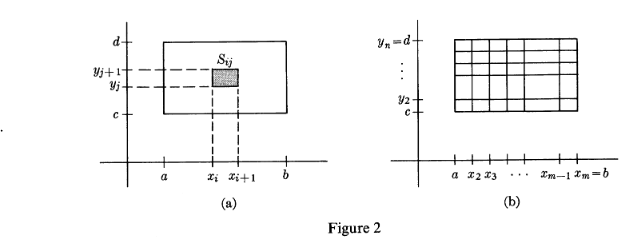
\includegraphics[scale = 0.8]{partition.PNG}
\end{figure}

We denote by $S_{ij}$ the subrectangle $[x_i,x_{i+1}] \times [y_j, y_{j+1}]$.

Double integrals are defined very similarly as in the single variable case.
\[U(f,P) = \sum_S (\sup_S f)(\area(S)),\ L(f,P)= \sum_S (\inf_S f)(\area(S)).\]

The double integral has two nice interpretations, one as a volume,
and the other as a mass.

In the same way the Riemann integral on an interval can handle
discontinuties as long as they are not too abundant, so too can
the Riemann integral on a region.
\textbf{Theorem.} Let $R$ be a rectangle and let $f$ be bounded on $R$
and continous except at possibly at points lying on a finite number
of curves. Then $f$ is integrable on $R$.

\end{document}
